% Sample Dissertation, Thesis, or Document %
%            for use with the              %
%  University of Arizona Thesis Class,     %
%               uathesis.cls               %
%------------------------------------------%

% We'll use the uathesis document class (duh).  The uncommented line
% below will produce a Dissertation, the others would produce a Thesis
% or a Document.  There are other options available to you like turning
% on the copyright statement and replacing the year on the title page
% with a "generated on" stamp (handy for early drafts).  To find out
% what the available options are, take a look into the uathesis.cls
% file and look for the \DeclareOption commands near the top of that
% file.
% There are five copyright options.  Copyright, no copyright, and three
% different Creative Commons licences.  Use the one you want (If you go
% Creative Commons, I (DM) think the CC-BY-ND makes the most sense)  See
% uathesis.cls for the reason why the non-commercial licenses are not
% included.
%\documentclass[dissertation]{uathesis}
\documentclass[dissertation,copyright]{uathesis}
%\documentclass[dissertation,CC-BY]{uathesis}
%\documentclass[dissertation,CC-BY-SA]{uathesis}
%\documentclass[dissertation,CC-BY-ND]{uathesis}
%\documentclass[dissertation,generatedon]{uathesis}
%\documentclass[thesis]{uathesis}
%\documentclass[document]{uathesis}

% Package Usage
% These are the packages that we need
%\usepackage{algorithm}
%\usepackage{algorithmic}
\usepackage{amsmath,amssymb,amsfonts}
\usepackage{algorithmic}

\usepackage[ruled,boxed,noend]{algorithm2e}
\usepackage{graphicx}
\usepackage{natbib}			% natbib is available on most systems, and is
					% terribly handy.
					% If you want to use a different Bibliography package, 
					% you should be able to, just change this
					% and the \bibliographystyle command below.  Be warned
					% that you may need to do a little hacking to get
					% the REFERENCES item to show up in your TOC.

\graphicspath{{figure/}{figures/}}
\usepackage[caption=false,font=footnotesize]{subfig}

% Compatibility with the AASTEX package 
% of the American Astronomical Society.
%\usepackage{deluxetable}		% Allows use of AASTEX deluxe tables
%\usepackage{aastex_hack}		% Allows other AASTEX functionality.

% These are other packages that you might find useful.
% For controlling the fonts, see
% http://www.math.uiuc.edu/~hartke/computer/latex/survey/survey.html
% The following is a nice font set:
%\usepackage{mathtime}			% Times for letters; Belleek math.
%
%\usepackage{amsmath}			% AMS Math (advanced math typesetti`ng)
%\usepackage{lscape}			% Used for making fitting large tables in by putting them landscape
%\usepackage{refs}			
%
% If you are using hyper-ref (recommended), this command must go after all 
% other package inclusions (from the hyperref package documentation).
% The purpose of hyperref is to make the PDF created extensively
% cross-referenced.
\usepackage[bookmarks,colorlinks=true,urlcolor=black,linkcolor=black,citecolor=black]{hyperref}

\usepackage[pages=some]{background}

\backgroundsetup{
scale=1,
%color=black,
opacity=0.5,
angle=0,
contents={%
  
\includegraphics[width=6.0in,height=6.0in]{UA-watermark.png}
  }%
}

\newcommand{\node}[1] {\textbf{#1}}

% Set up some values.
\completetitle{My Title}
\fullname{My Name} % Grad college wants your full name here.
\degreename{Doctor of Philosophy}	% Title of your degree.

\begin{document}

% Set up the title page
\maketitlepage
{DEPARTMENT OF COMPUTER SCIENCE}	% Title of your department.
{2022}							

% Insert the approval form.  Note that for electronic submission
% of your Ph. D. dissertation, you must bring *two* copies of the
% approval page to your final defense.  These must be signed by
% the committee.  Make two photocopies: one for Pam and the other
% for your records.  Then, bring the two signed originals to the
% graduate college when you submit the final version of the
% dissertation to the University of Arizona.
\approval
{XX March 2022}		  % Sign-off Date	
{Computer Science}	% Academic Department
{Member A}		% Dissertation Director
{Member A}    % 1st committee member, mostly same as Director/Chair
{Member B}		% 2nd committee member
{Member C}		  % 3rd committee member
{Member D}		    % 4th committee member
%{} % 5th committee member (leave empty if None)
\BgThispage

% Include the ``Acknowledgements''
\incacknowledgements{acknowledgements}

% Include the ``Dedication''
\incdedication{dedication}

% Create a ``Table of Contents''
\tableofcontents

% Create a ``List of Figures''
\listoffigures

% Create a ``List of Tables''
\listoftables

% Include the ``Abstract''
\incabstract{abstract}

% Include the various chapters
\chapter{INTRODUCTION}
\label{chapter:introduction}

Contactless payments also known as Near Field Communication \cite{want2011near} (NFC) payments is getting more 
and more popular throughout the world. In 2019, the global NFC market size was valued at \$15 million and the 
projection shows that by 2028 it will reach \$54 million \cite{nfcmarket}. Moreover, the COVID-19 pandemic has 
significantly increased the use of contactless payments \cite{contactlesscovid}. 
To make a contactless payment, one needs to own a contactless-enabled card which can be used near a NFC Point of 
Sale (POS). Also, major phone vendors like Google, Samsung, Apple has started manufacturing NFC-enabled smart 
devices which can be used to make a contactless payment. Digital NFC-wallet applications can be installed and 
activated with a contactless credit/debit card and then used to make a transaction near a contactless-supported 
terminal.  

Since Android 4.4 introduced Host based card emulation \cite{hostbased} which allows an Android application to 
emulate a card and communicate directly with an NFC reader, bypassing the necessity of a Secure Element (SE), 
developers can now build digital NFC-wallet extending Android's Host Apdu Service class\cite{hostapdu}. Among the 
available NFC-wallets, Google Pay\cite{gpay} and Apple Pay are the most prominent wallet applications being used 
widely. In addition to these third party applications, many banks develop their own digital wallet application for 
their customers. To build such an application, the developers follow the standard protocol described by 
EMV (Europay Mastercard Visa)\cite{van2016emv}. 

Recent works have shown that EMV contactless payment protocol \cite{emvco} has vulnerabilities that can be 
exploited to make an unauthorized purchase \cite{emms2016contactless}\cite{francis2009potential}. 
\citet{emvandvulnerabilities} presented an overview of the EMV protocol and how it's vulnerable to different 
types of security attacks. However, the focus of previous research work in this field is on the protocol itself, 
rather than the implementation of the protocol. We are interested in verifying the protocol implementation to 
ensure that the EMV specifications are properly followed by NFC-wallet applications' developers.

PayFuzz aims to find the gap between the EMV protocol specification and it's implementation on real-life wallet 
applications. We feed the wallet payment interface with our constructed commands and record the response to 
create a finite state machine(FSM) using LearnLib similar to \cite{formalmodels}. Discrepancies between state 
machines from different wallet applications move us to the evaluation stage where we find vulnerabilities in 
the implementation which can be leveraged to launch an attack on the wallet application. Specifically, the goal is to 
develop rigorous techniques for formally studying the security and compliance issues of payment applications 
(wallets and POS) with automated reasoning (i.e., formal methods and program analysis) and build defenses. We also 
aim to create formal specifications and enable secure code generation for critical components as a long-term goal.



In this work, to extract a behavioral abstraction from NFC wallets, we use an active automata learning approach \cite{dikeue} 
\cite{dynamictesting}. 

\chapter{Example Chapter}
\label{chapter:example-chapter}

An example chapter.

\section{Sub-chapter section A}
\label{section:example-sectionA}

Example Figure~\ref{fig:sample-figure},

\begin{figure}[!ht]
  \centering
  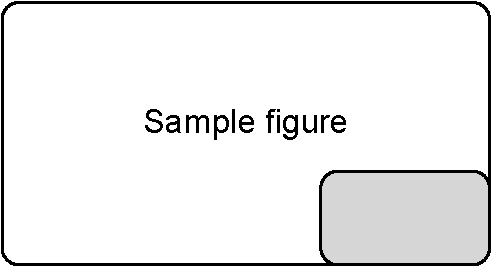
\includegraphics[height=0.25\textwidth]{sample-figure.pdf}
  \caption{Sample Figure.}
  \label{fig:sample-figure}
\end{figure}
\section{Sub-chapter section B}
\label{section:example-sectionB}

Some random text...
\chapter{CONCLUSION}
\label{chapter:conclusion}

Some conclusion

% Include the various appendices
% \appendix
% \chapter{Sample Appendix}
\label{apndxA}
Stuff.....



% Switch the spacing to single-spaced for the references
\renewcommand{\baselinestretch}{1}		% changing the value
\small\normalsize										% switch size to make the value take

% Create the References list
\bibliographystyle{uabibnat}
\bibliography{bibliography}

\end{document}
